%%%%%%%%%%%%%%%%%%%%%%%%%%%%%%%%%%%%%%%%%
% Short Sectioned Assignment LaTeX Template Version 1.0 (5/5/12)
% This template has been downloaded from: http://www.LaTeXTemplates.com
% Original author:  Frits Wenneker (http://www.howtotex.com)
% License: CC BY-NC-SA 3.0 (http://creativecommons.org/licenses/by-nc-sa/3.0/)
%%%%%%%%%%%%%%%%%%%%%%%%%%%%%%%%%%%%%%%%%

%----------------------------------------------------------------------------------------
%	PACKAGES AND OTHER DOCUMENT CONFIGURATIONS
%----------------------------------------------------------------------------------------

\documentclass[paper=a4, fontsize=10pt]{scrartcl} % A4 paper and 11pt font size

% ---- Entrada y salida de texto -----

\usepackage[T1]{fontenc} % Use 8-bit encoding that has 256 glyphs
\usepackage[utf8]{inputenc}
\usepackage{blindtext}
%\usepackage{fourier} % Use the Adobe Utopia font for the document - comment this line to return to the LaTeX default

% ---- Idioma --------

\usepackage[spanish, es-tabla]{babel} % Selecciona el español para palabras introducidas automáticamente, p.ej. "septiembre" en la fecha y especifica que se use la palabra Tabla en vez de Cuadro

% ---- Otros paquetes ----

\usepackage{amsmath,amsfonts,amsthm} % Math packages
%\usepackage{graphics,graphicx, floatrow} %para incluir imágenes y notas en las imágenes
\usepackage{graphics,graphicx, float} %para incluir imágenes y colocarlas
\usepackage{color}
\usepackage{amsmath}
% Para hacer tablas comlejas
%\usepackage{multirow}
%\usepackage{threeparttable}
\definecolor{dkgreen}{rgb}{0,0.6,0}
%\usepackage{sectsty} % Allows customizing section commands
%\allsectionsfont{\centering \normalfont\scshape} % Make all sections centered, the default font and small caps
\definecolor{gray}{rgb}{0.5,0.5,0.5}
\definecolor{mauve}{rgb}{0.58,0,0.82}
\usepackage{fancyhdr} % Custom headers and footers
\usepackage{url} % Custom headers and footers
\pagestyle{fancyplain} % Makes all pages in the document conform to the custom headers and footers
\fancyhead{} % No page header - if you want one, create it in the same way as the footers below
\fancyfoot[L]{} % Empty left footer
\usepackage{hyperref}
\usepackage{listings}
\fancyfoot[C]{} % Empty center footer
\fancyfoot[R]{\thepage} % Page numbering for right footer
\renewcommand{\headrulewidth}{0pt} % Remove header underlines
\renewcommand{\footrulewidth}{0pt} % Remove footer underlines
\setlength{\headheight}{12pt} % Customize the height of the header
\usepackage[
	type={CC},
	modifier={by-nc-sa},
	version={3.0},
]{doclicense}

\lstset{frame=tb,
	language=C,
	aboveskip=3mm,
	belowskip=3mm,
	showstringspaces=false,
	columns=flexible,
	basicstyle={\small\ttfamily},
	numbers=none,
	numberstyle=\tiny\color{gray},
	keywordstyle=\color{blue},
	commentstyle=\color{dkgreen},
	stringstyle=\color{mauve},
	breaklines=true,
	breakatwhitespace=true,
	tabsize=3
}

\setlength\parindent{0pt} % Removes all indentation from paragraphs - comment this line for an assignment with lots of text

\newcommand{\horrule}[1]{\rule{\linewidth}{#1}} % Create horizontal rule command with 1 argument of height


%----------------------------------------------------------------------------------------
%	TÍTULO Y DATOS DEL ALUMNO
%----------------------------------------------------------------------------------------

\title{	
\normalfont \normalsize 
\textsc{{ Estructura de datos (2017-2018)} \\ Grado en Ingeniería Informática \\ Universidad de Granada} \\ [25pt] % Your university, school and/or department name(s)
\huge Práctica 1: eficiencia  \\ % The assignment title
}
\author{Manuel Jiménez Bernal}
\date{\normalsize\today} % Incluye la fecha actual

%----------------------------------------------------------------------------------------
% DOCUMENTO
%----------------------------------------------------------------------------------------

\begin{document}

\maketitle % Muestra el Título

Esta práctica se ha realizado en un equipo de siguientes prestaciones:
\begin{itemize}  
	\item 24 GB de Memoria RAM DDR3 
	\item Procesador Intel Core i7-2600 @ 3.40 Ghz
	\item Entorno en una máquina virtual bajo GNU/Linux: Ubuntu 16.04
\end{itemize}

Todos los códigos fuente de los ejercicios abajo descritos se proporcionan en un directorio adjunto, así como cualquier script o imagen que se ha utilizado.

\section{Ejercicio 1: Ordenación de la burbuja}

Al tratarse de dos bucles anidados en función de N, puede hablarse de que la eficiencia teórica de este algoritmo es de clasificación cuadrática: \[ \dfrac{ n^2 - n}{2} \]
En notación O (peor caso): $O(n^2)$ % regular O

Para automatizar la ejecución del algoritmo se preparó un script que invoca el programa compilado con parámetros incrementales.

\begin{lstlisting}
#!/bin/csh
@ inicio = 100
@ fin = 30000
@ incremento = 500
set ejecutable = burbuja
set salida = tiempos_burbuja.dat

@ i = $inicio
echo > $salida
while ( $i <= $fin )
echo Ejecucion tam = $i
echo `./{$ejecutable} $i 10000` >> $salida
@ i += $incremento
end
\end{lstlisting}

Esta ejecución genera un fichero con los tiempos obtenidos a partir de los distintos valores de tamaño a la hora de crear el vector. Con la herramienta gnuplot se generó una gráfica de puntos a partir de estos datos. Con el siguiente comando:

\begin{lstlisting}
>plot 'tiempos_burbuja.dat'
\end{lstlisting}

Se genera el siguiente gráfico:

\begin{figure}[H] %con el [H] le obligamos a situar aquí la figura
	\centering
	\label{lsblk}
	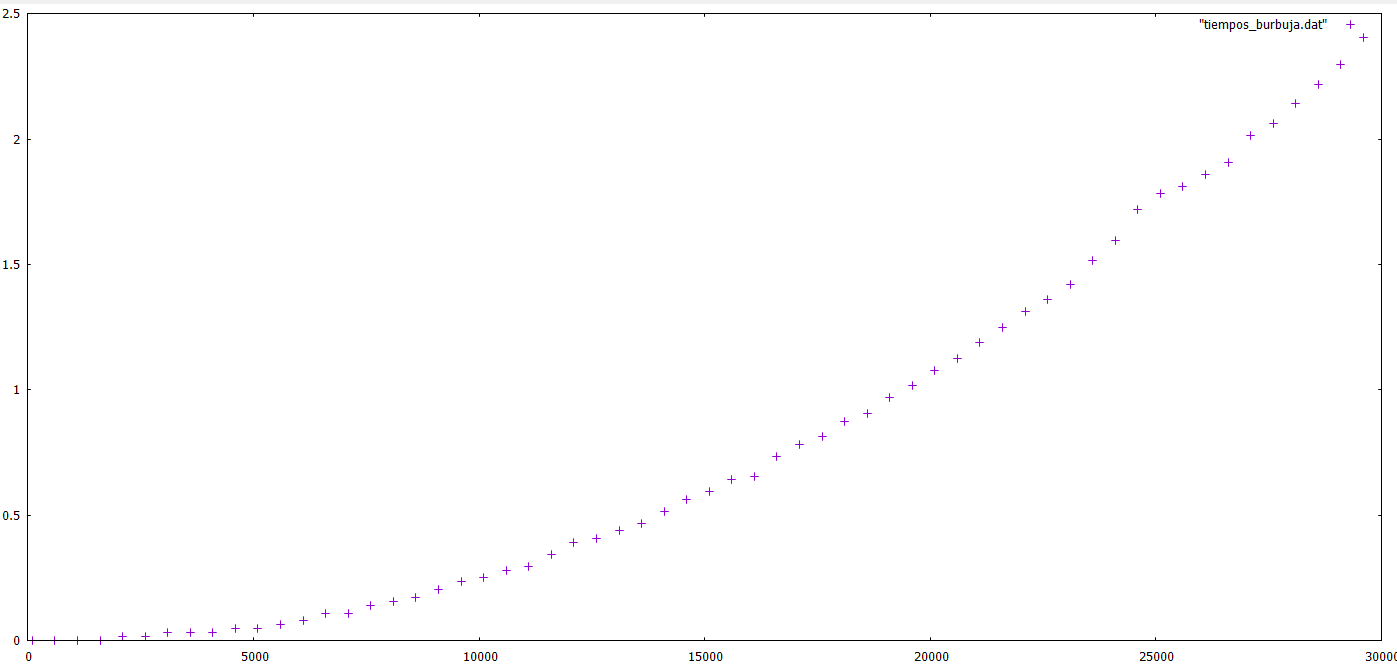
\includegraphics[width=0.8\textwidth]{../imgs/c1.PNG}
	\caption{Gráfica de puntos a partir de los datos del fichero tiempos\_burbuja.dat} 
\end{figure}

Con la siguiente secuencia de gnuplot puede visualizarse la comparativa gráfica entre los datos de la eficiencia teórica con respecto a la eficiencia empírica:

\begin{lstlisting}
set xrange [0 : 30000]
set x2range [0 : 3000]
set yrange [0 : 3]
set y2range [0 : 5000000]
plot 'tiempos\_burbuja.dat' axes x1y1, (x*x-x)/2 axes x2y2
\end{lstlisting}
\begin{figure}[H] %con el [H] le obligamos a situar aquí la figura
	\centering
	\label{lsblk}
	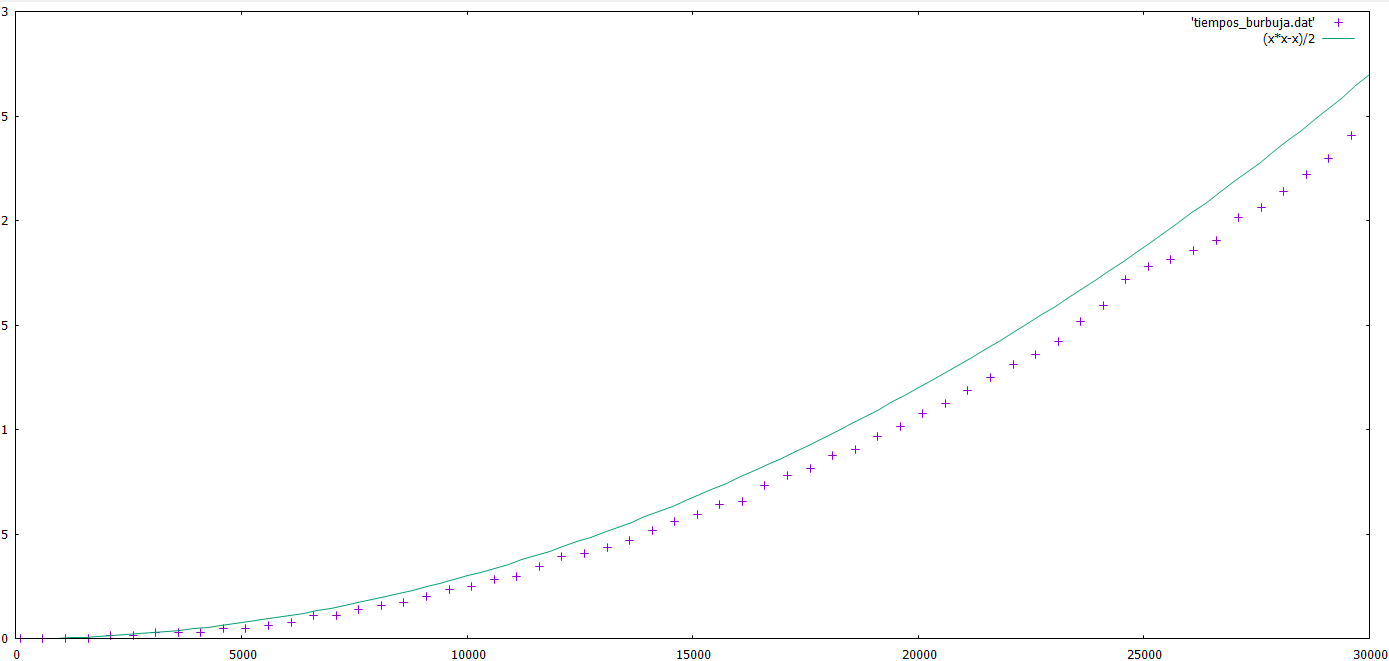
\includegraphics[width=0.8\textwidth]{../imgs/c2.PNG}
	\caption{Puede decirse que la eficiencia empírica se ajusta a la eficiencia teórica.} 
\end{figure}

Fue necesario ajustar los límites de la función f(x) debido a los bajos tiempos de ejecución provocaban que la visualización se distorsionase al verse de forma horizontal, condicionados por los altos valores de f(x) y estar ambas compartiendo los ejes.

\section{ Ejercicio 2: Ajuste en la ordenación de la burbuja}

Se realizaron los siguientes comandos de gnuplot:

\begin{lstlisting}
f(x) = (a*x)**2 + b*x + c
fit f(x) "tiempos_burbuja.dat" via a, b, c
\end{lstlisting}

Tras lo cual se generó un fichero 'fit.log', el cual proporciona la información extraída de la interpolación por mínimos cuadrados:

\begin{lstlisting}
Thu Sep 28 20:31:15 2017
FIT:    data read from 'tiempos_burbuja.dat'
format = z
#datapoints = 60
residuals are weighted equally (unit weight)

function used for fitting: f(x)
f(x) = a*x**2 + b*x + c
fitted parameters initialized with current variable values

iter      chisq       delta/lim  lambda   a             b             c            
0 9.4779953826e+18   0.00e+00  2.29e+08    1.000000e+00   1.000000e+00   1.000000e+00
12 9.4804551914e-04  -4.34e-05  2.29e-04    2.841925e-09  -3.242199e-06   9.435810e-04

After 12 iterations the fit converged.
final sum of squares of residuals : 0.000948046
rel. change during last iteration : -4.33886e-10

degrees of freedom    (FIT_NDF)                        : 57
rms of residuals      (FIT_STDFIT) = sqrt(WSSR/ndf)    : 0.00407828
variance of residuals (reduced chisquare) = WSSR/ndf   : 1.66324e-05

Final set of parameters            Asymptotic Standard Error
=======================            ==========================
a               = 2.84192e-09      +/- 7.854e-12    (0.2764%)
b               = -3.2422e-06      +/- 2.411e-07    (7.435%)
c               = 0.000943581      +/- 0.001549     (164.2%)

correlation matrix of the fit parameters:
a      b      c      
a               1.000 
b              -0.968  1.000 
c               0.738 -0.861  1.000 
\end{lstlisting}

De estos datos se extrae que: 
\[
f(n) = 2.84192^{-9}n^2 -3.2422^{-6}n + 0.000943581
\]

Al realizar el ajuste se obtiene el siguiente gráfico:

\begin{figure}[H] %con el [H] le obligamos a situar aquí la figura
	\centering
	\label{lsblk}
	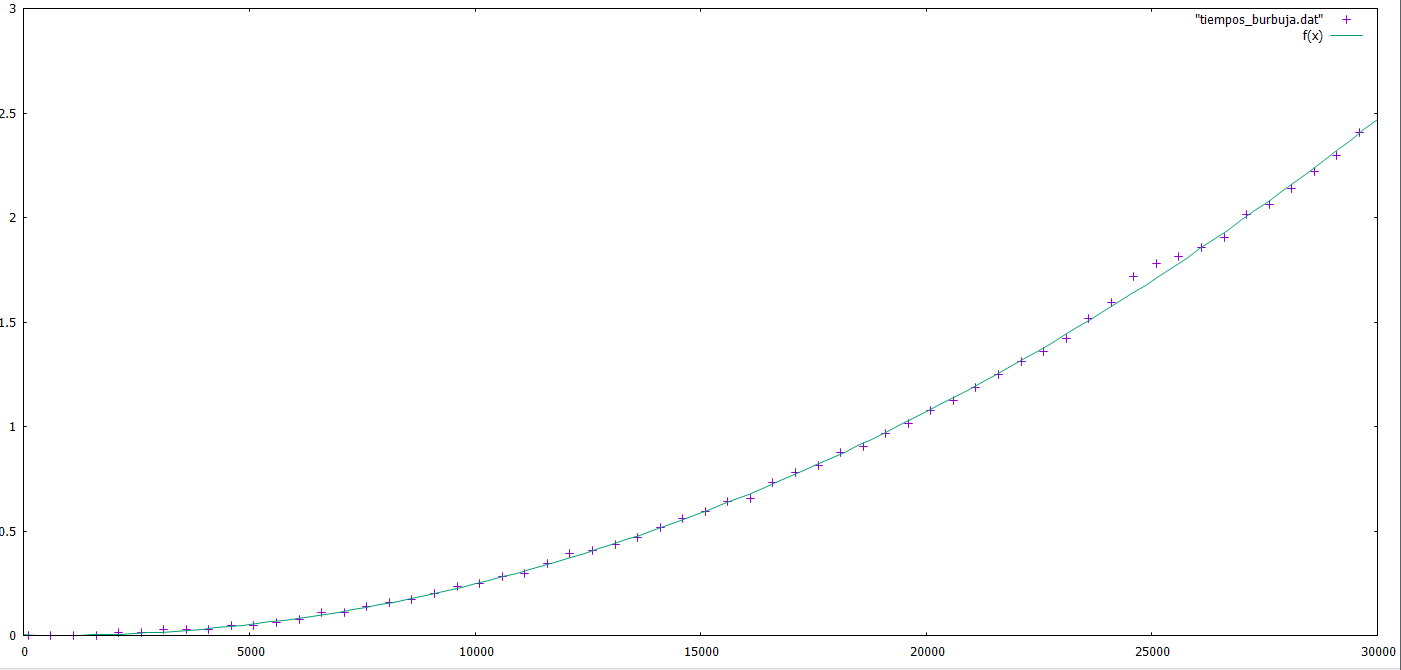
\includegraphics[width=0.8\textwidth]{../imgs/c3.PNG}
	\caption{Ajuste por regresión de los datos obtenidos} 
\end{figure}

\section{Ejercicio 3:  Problemas de precisión}

Se trata de un algoritmo de búsqueda binaria para un vector de números ya ordenados. El algoritmo acota la búsqueda en función del valor del número en casa posición, y divide a la mitad el tamaño del problema en las sucesivas iteraciones. En el programa se fuerza el peor caso pasando como argumento un número que no existe en el array.

\subsection{Ejercicio 3:  Eficiencia teórica}

En el peor caso el vector puede dividirse tantas veces como subconjuntos de mitades pueda hacerse de cada uno de esos subconjuntos iterativamente. Este comportamiento implica una eficiencia de orden logarítmico  $O(log_2(n))$ % regular O

\begin{figure}[H] %con el [H] le obligamos a situar aquí la figura
	\centering
	\label{lsblk}
	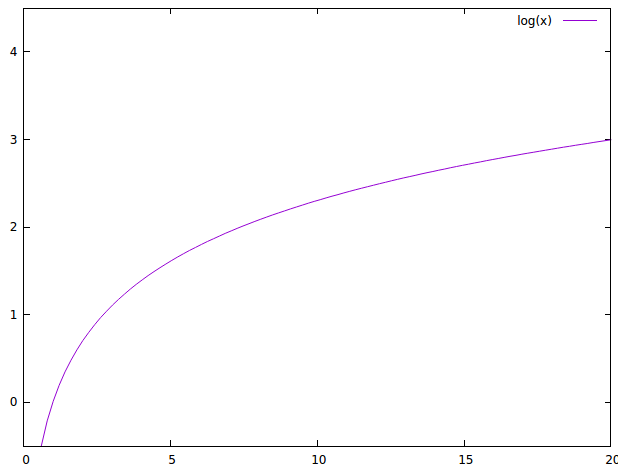
\includegraphics[width=0.8\textwidth]{../imgs/ej3logteoric.PNG}
	\caption{Eficiencia teórica} 
\end{figure}

\subsection{Ejercicio 3:  Eficiencia empírica}

Para medir los tiempos empíricos de este algoritmo se ha realizado un script con el que generar de forma automática vectores de tamaños distintos en cada iteración, tras extraer estos datos se dibujaron gráficas en gnuplot:

\begin{figure}[H] %con el [H] le obligamos a situar aquí la figura
	\centering
	\label{lsblk}
	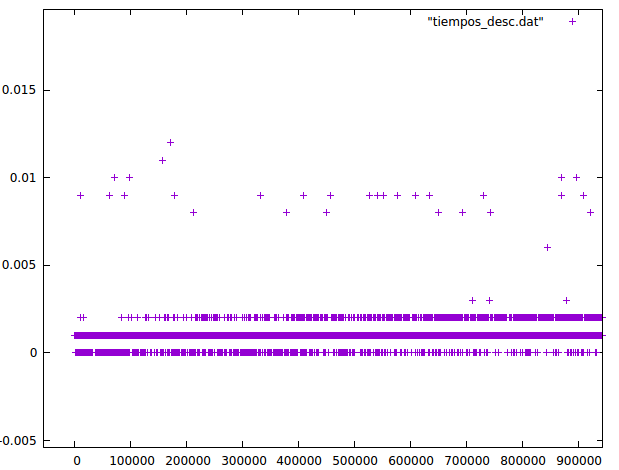
\includegraphics[width=0.8\textwidth]{../imgs/ejercicio3b.PNG}
	\caption{Eficiencia empírica} 
\end{figure}

Como se aprecia en la gráfica hay una anomalía en la representación, ya que eventualmente los tiempos se disparan de forma muy irregular.
Tras realizar los siguientes comandos en gnuplot el ajuste por regresión resultó de la siguiente manera:

\begin{lstlisting}
gnuplot> f(x) = a*x**2 + b*x + c
gnuplot> fit f(x) 't.txt' via a,b,c
\end{lstlisting}

Arrojando el siguiente ajuste:

\begin{lstlisting}
Final set of parameters            Asymptotic Standard Error
=======================            ==========================
a               = -4.81698e-09     +/- 4.687e-10    (9.729%)
b               = 1                +/- 0.1258       (12.58%)
c               = 1                +/- 7.084e+06    (7.084e+08%)

correlation matrix of the fit parameters:
a      b      c      
a               1.000 
b              -0.968  1.000 
c               0.748 -0.868  1.000 
\end{lstlisting}

\begin{figure}[H] %con el [H] le obligamos a situar aquí la figura
	\centering
	\label{lsblk}
	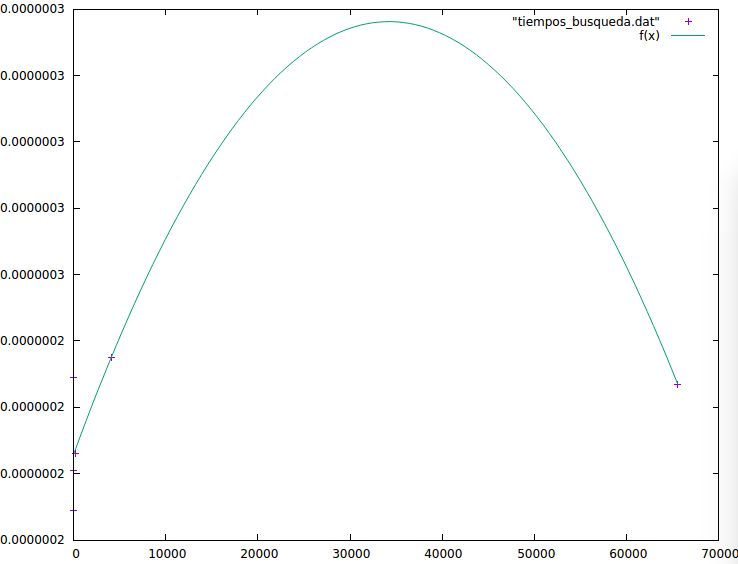
\includegraphics[width=0.8\textwidth]{../imgs/ejercicio3c.PNG}
	\caption{Ajuste de eficiencia empírica y teórica} 
\end{figure}

En el gráfico se aprecia cómo debido a las irregularidades de los resultados se hace un ajuste que no es el que se esperaba conseguir, ya que el tiempo parece constante.

\section{Ejercicio 4:  Mejor y peor caso}
Se modificó el código fuente del algoritmo de la burbuja para permitir introducir mediante parámetro el modo mejor o peor caso, proporcionando un vector ya ordenado o el inverso.
Antes de realizar modificaciones la ejecución por lotes mostraba los siguientes resultados de tiempo:
Tras ejecutar los scripts que ejecutan de forma iterativa e incremental el programa, se procesaron los resultados en gnuplot con los siguientes resultados:

\begin{figure}[H] %con el [H] le obligamos a situar aquí la figura
	\centering
	\label{lsblk}
	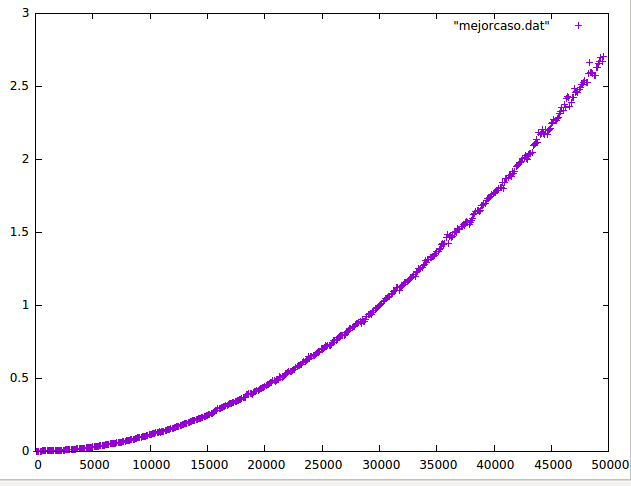
\includegraphics[width=0.8\textwidth]{../imgs/ejercicio4a.PNG}
	\caption{Gráfica de puntos a partir de los datos de ejecución del algoritmo forzando el mejor caso} 
\end{figure}

\begin{figure}[H] %con el [H] le obligamos a situar aquí la figura
	\centering
	\label{lsblk}
	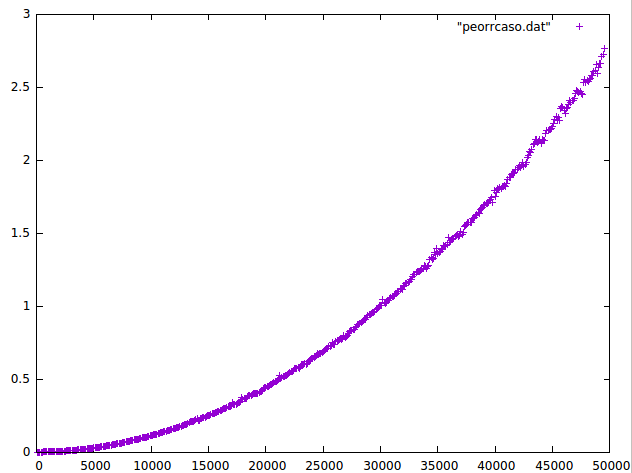
\includegraphics[width=0.8\textwidth]{../imgs/ejercicio4c.PNG}
	\caption{Gráfica de puntos a partir de los datos de ejecución del algoritmo forzando el peor caso} 
\end{figure}

La representación de la comparación en los dos escenarios descritos anteriormente:

\begin{figure}[H] %con el [H] le obligamos a situar aquí la figura
	\centering
	\label{lsblk}
	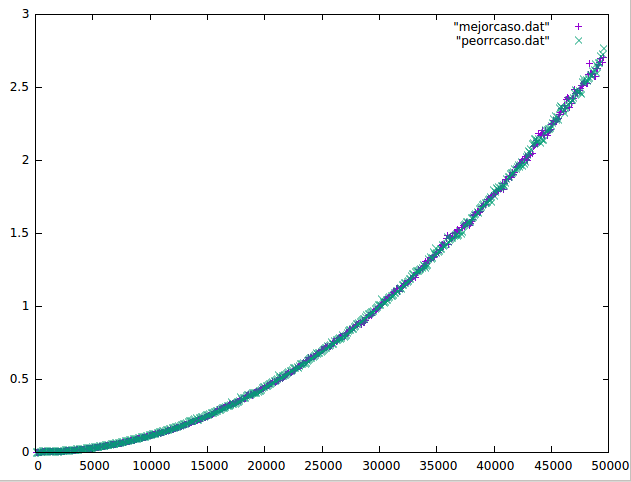
\includegraphics[width=0.8\textwidth]{../imgs/ejercicio4b.PNG}
	\caption{Mejor y peor caso} 
\end{figure}

La conclusión que se extrae es que la ganancia en velocidad al proporcionar un vector ya ordenado apenas es perceptible, ya que de esta forma lo único que se ahorran son comparaciones y asignaciones que en conjunto es de una eficiencia constante u $O(1)$, el número de iteraciones es el mismo. 

\section{Ejercicio 5}

Al introducir el cambio y encontrarse el vector ya ordenado, el algoritmo entra únicamente en la primera iteración al bucle exterior, recorriendo el bucle interior de forma completa una sola vez. Por tanto se trata de una eficiencia lineal $O(n)$.

\begin{figure}[H] %con el [H] le obligamos a situar aquí la figura
	\centering
	\label{lsblk}
	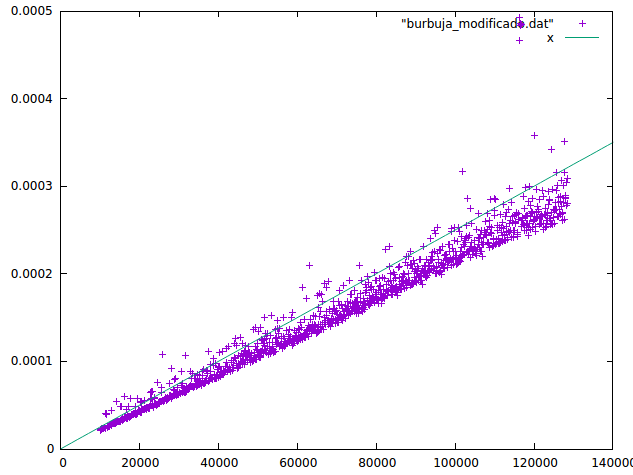
\includegraphics[width=0.8\textwidth]{../imgs/ejercicio5.PNG}
	\caption{Gráfica a partir de los datos proporcionando un vector ya ordenado y habiendo modificado el algoritmo} 
\end{figure}

Tras observar la gráfica puede afirmarse que la eficiencia teórica y práctica se ajustan considerablemente.
\section{Ejercicio 6}
Se compiló el programa con el algoritmo de la burbuja con parámetros de optimización -O3 y los resultados en tiempo de las prestaciones fueron los siguientes tras modelar los datos en gnuplot:

\begin{figure}[H] %con el [H] le obligamos a situar aquí la figura
	\centering
	\label{lsblk}
	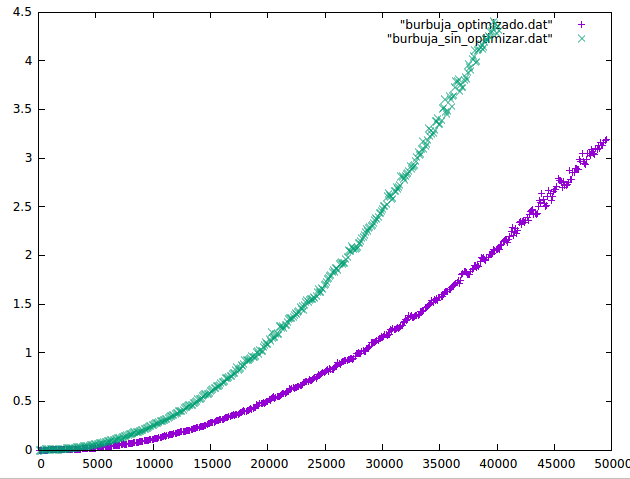
\includegraphics[width=0.8\textwidth]{../imgs/ejercicio6.PNG}
	\caption{Algoritmo de la burbuja con optimización -O3} 
\end{figure}

Por tanto puede afirmarse que se consigue una ganancia notable en velocidad utilizando optimización en el compilador.

\end{document}





